\documentclass[20pt,letterpaper]{article}
\usepackage[utf8]{inputenc}
\usepackage{physics}
\usepackage{fancyhdr}
\usepackage{amsmath}
\usepackage{cancel}
\usepackage{graphicx}
\usepackage{graphics}
\usepackage{extarrows}
\usepackage{caption}
\usepackage{subcaption}
\usepackage[margin=1in]{geometry}
\usepackage[version=4]{mhchem}
\usepackage{mathtools}
\usepackage{amsfonts}
\usepackage{amsmath}
\usepackage{amssymb}
\usepackage{xcolor}
\usepackage{sectsty}
\usepackage{ulem}
\usepackage{hyperref}
\usepackage{pgfplots}
\usepackage{mathrsfs}
\usepackage{pythonhighlight}
\newcommand*{\hatH}{\hat{\mathcal{H}}}
\newcommand*{\hatD}{\hat{\mathcal{D}}}
\pagestyle{fancy}
\fancyhf{}
\rhead{Physics 129L HW 5}
\lhead{Jin \thepage}

\begin{document}
	\uline{Name:} Chang Jin
\section{Problem 1}
Running Running the \textbf{ls -alF} command on the top level directory of the flash drive:\\
\textbf{Output:} included in the txt file: \textit{Problem\_1\_outputs\_a.txt}\\
Running the \textbf{ls -alF} command on the top level directory of the most recent backup on the flash drive:\\
\textbf{Output:} included in the txt file: \textit{Problem\_1\_outputs\_b.txt}
\section{Problem 2}
Using \textbf{diff} command on the python code use to solve Problem 3 and \textbf{img.py} we have the output:\\
included in the .txt file: \textit{Problem\_2\_outputs.txt}

\section{Problem 3}
The relevant code is included in the file \textit{Problem\_3.py}\\
Steps for graphing the triangle in an image file that is 512 pixels by 512 pixels:
\begin{itemize}
	\item First, we set the entire image as blue
	\item Second, set the pixels at the boundary of the image to white with code:
	\begin{python}
		# 
		# set the border pixels to white (requirement 1)
		# 
		borderbottom1 = 0
		bordertop1 = int(Y/10)
		borderbottom2 = int(Y-Y/10)
		bordertop2 = Y
		borderbottom3 = 0
		bordertop3 = int(X/10)
		bordertop4 = X
		borderbottom4 = int(X-X/10)
		
		pvals[:,borderbottom1:bordertop1,:] = (0xff,0xff,0xff)  # white
		pvals[:,borderbottom2:bordertop2,:] = (0xff,0xff,0xff)  # white
		pvals[borderbottom3:bordertop3,:,:] = (0xff,0xff,0xff)  # white
		pvals[borderbottom4:bordertop4,:,:] = (0xff,0xff,0xff)  # white
	\end{python}
	\item Then set the pixels that is above the line $y = (3/4)\cdot x$ to white with the code (note, we only need to set the red and green plane to 255 because the blue plane is already 255):
	\begin{python}
		for j in range(Y):
			for i in range(X):
				if j>i*(3/4):
					pvals[i,j,0] = 0xff  # red
					pvals[i,j,1] = 0xff    # green
	\end{python}
	this gives us a filled 3-4-5 blue triangle.
	\item Next, we need to cut a triangle within the filled 3-4-5 triangle by setting these pixels specified by the code to white:
	\begin{python}
		for j in range(Y):
			for i in range(X):
				if j<=(i*(3/4)-Y//15) and (j>(bordertop1+Y//20)) and (i<(Y-(bordertop3+Y//20))):
					pvals[i,j,0] = 0xff  # red
					pvals[i,j,1] = 0xff  # green
	\end{python}
we can adjust the thickness of the triangle by changing the denominators for the parameters $Y//20$ and $Y//15$
\end{itemize}
the resulting 3-4-5 triangle:
\begin{figure*}[h]
	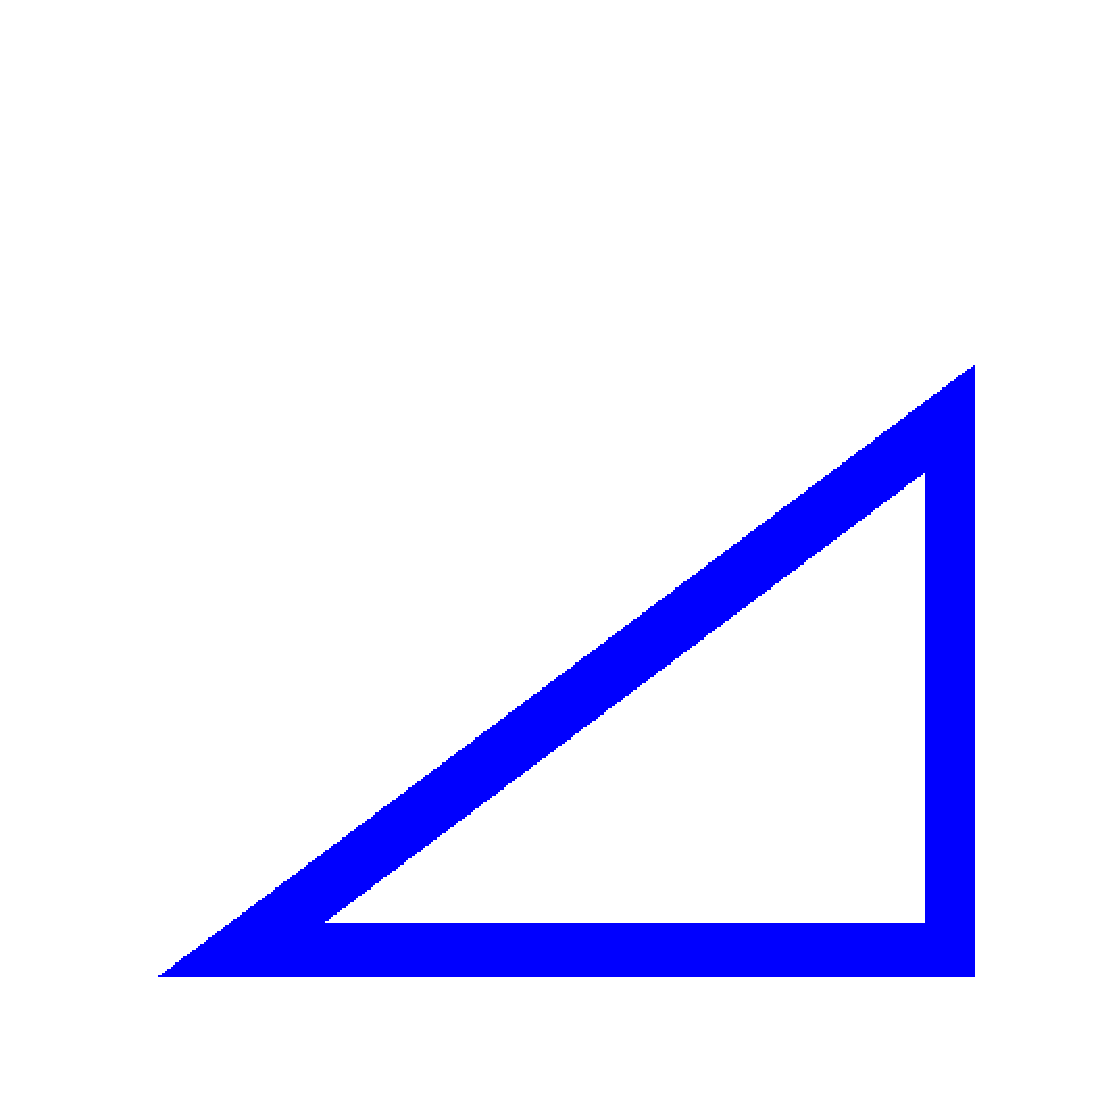
\includegraphics[scale=0.35]{Problem3}
\end{figure*}
\section{Problem 4}
From \href{https://en.wikipedia.org/wiki/Mandelbrot_set}{Wikipedia}, we see that for $c$ to be in the Mandelbrot set, $\mid z_n^2 + c \mid$ can never exceed 2. Hence we can set the limit to 2. \\
Using the code included in \textit{Problem\_4.py} we can plot the corresponding graph. 
\begin{figure*}[h]
	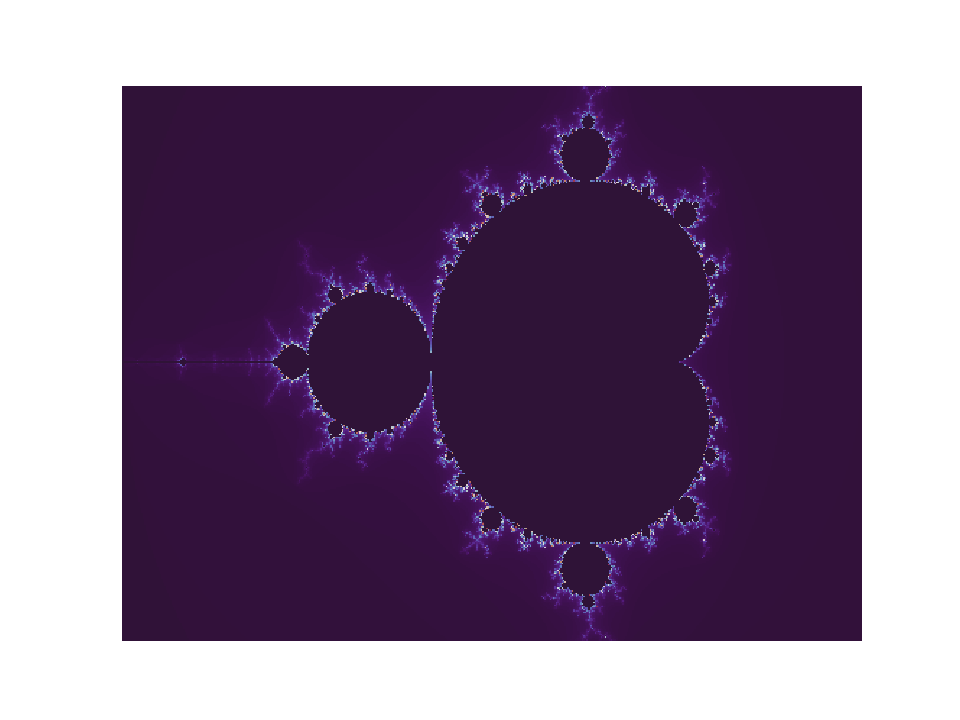
\includegraphics[scale=0.75]{Problem4}
\end{figure*}
Note: the image is saved as \textit{Problem4.pdf} in the folder.
\section{Problem 5}
The relevant code is included in \textit{Problem5.py}\\
Using the equation we obtained from \href{https://www.sciencedirect.com/topics/engineering/airy-disk}{ScienceDirect}:
\begin{equation*}
	PSF (r') = [2\frac{J_1(r')}{r'}]^2
\end{equation*}
where the normalized radius $r'$ is given by 
\begin{equation*}
	r' = \frac{\pi D}{\lambda f}r
\end{equation*}
where
\begin{align*}
	D &= \text{ aperature diameter} \\
	f &= \text{focal length} \\
	\lambda &= \text{wavelength of light} \\
	J_1 &= \text{Bessel function of the first kind to the first order}
\end{align*}
Assuming the focal length of the telescope is $1 m$ and we are looking at light in the IR regime with wavelength $\lambda = 700 nm$ and the diameter of the lens used is $ 10 m$, then we can plot the normalized peak as
\begin{figure*}[h]
	\includegraphics[scale=1]{Problem5}
	\caption{Linear z-scale}
\end{figure*}
\begin{figure*}[h]
	\includegraphics[scale=1]{Problem5 (zlog)}
	\caption{Log z-scale}
\end{figure*}
where 
\begin{align*}
	x &= \cos(\theta)r \\
	y&= \sin(\theta)r
\end{align*}
\end{document}
